
% Miranda's veil chapter ----------------------------------------------
\chapter*{Miranda's veil}
\addcontentsline{toc}{chapter}{Miranda's veil}

\begin{flushright}
\parbox{0.8\textwidth}{
\emph{Under all that we think, lives all we believe, like the ultimate veil of our spirits. \\
\hspace*{\fill}{\textperiodcentered \textperiodcentered \textperiodcentered \hspace*{0.2em} Antonio Machado} } }
\end{flushright}

\noindent
Miranda's veil is chess variant which is played on 16 x 16 board, with
white and dark violet fields and light magenta and indigo pieces. In
algebraic notation, columns are enumerated from 'a' to 'p', and rows
are enumerated from '1' to '16'. A new piece is introduced, Wave.

\clearpage % ..........................................................

\section*{Wave}
\addcontentsline{toc}{section}{Wave}

\noindent
\begin{wrapfigure}[12]{l}{0.4\textwidth}
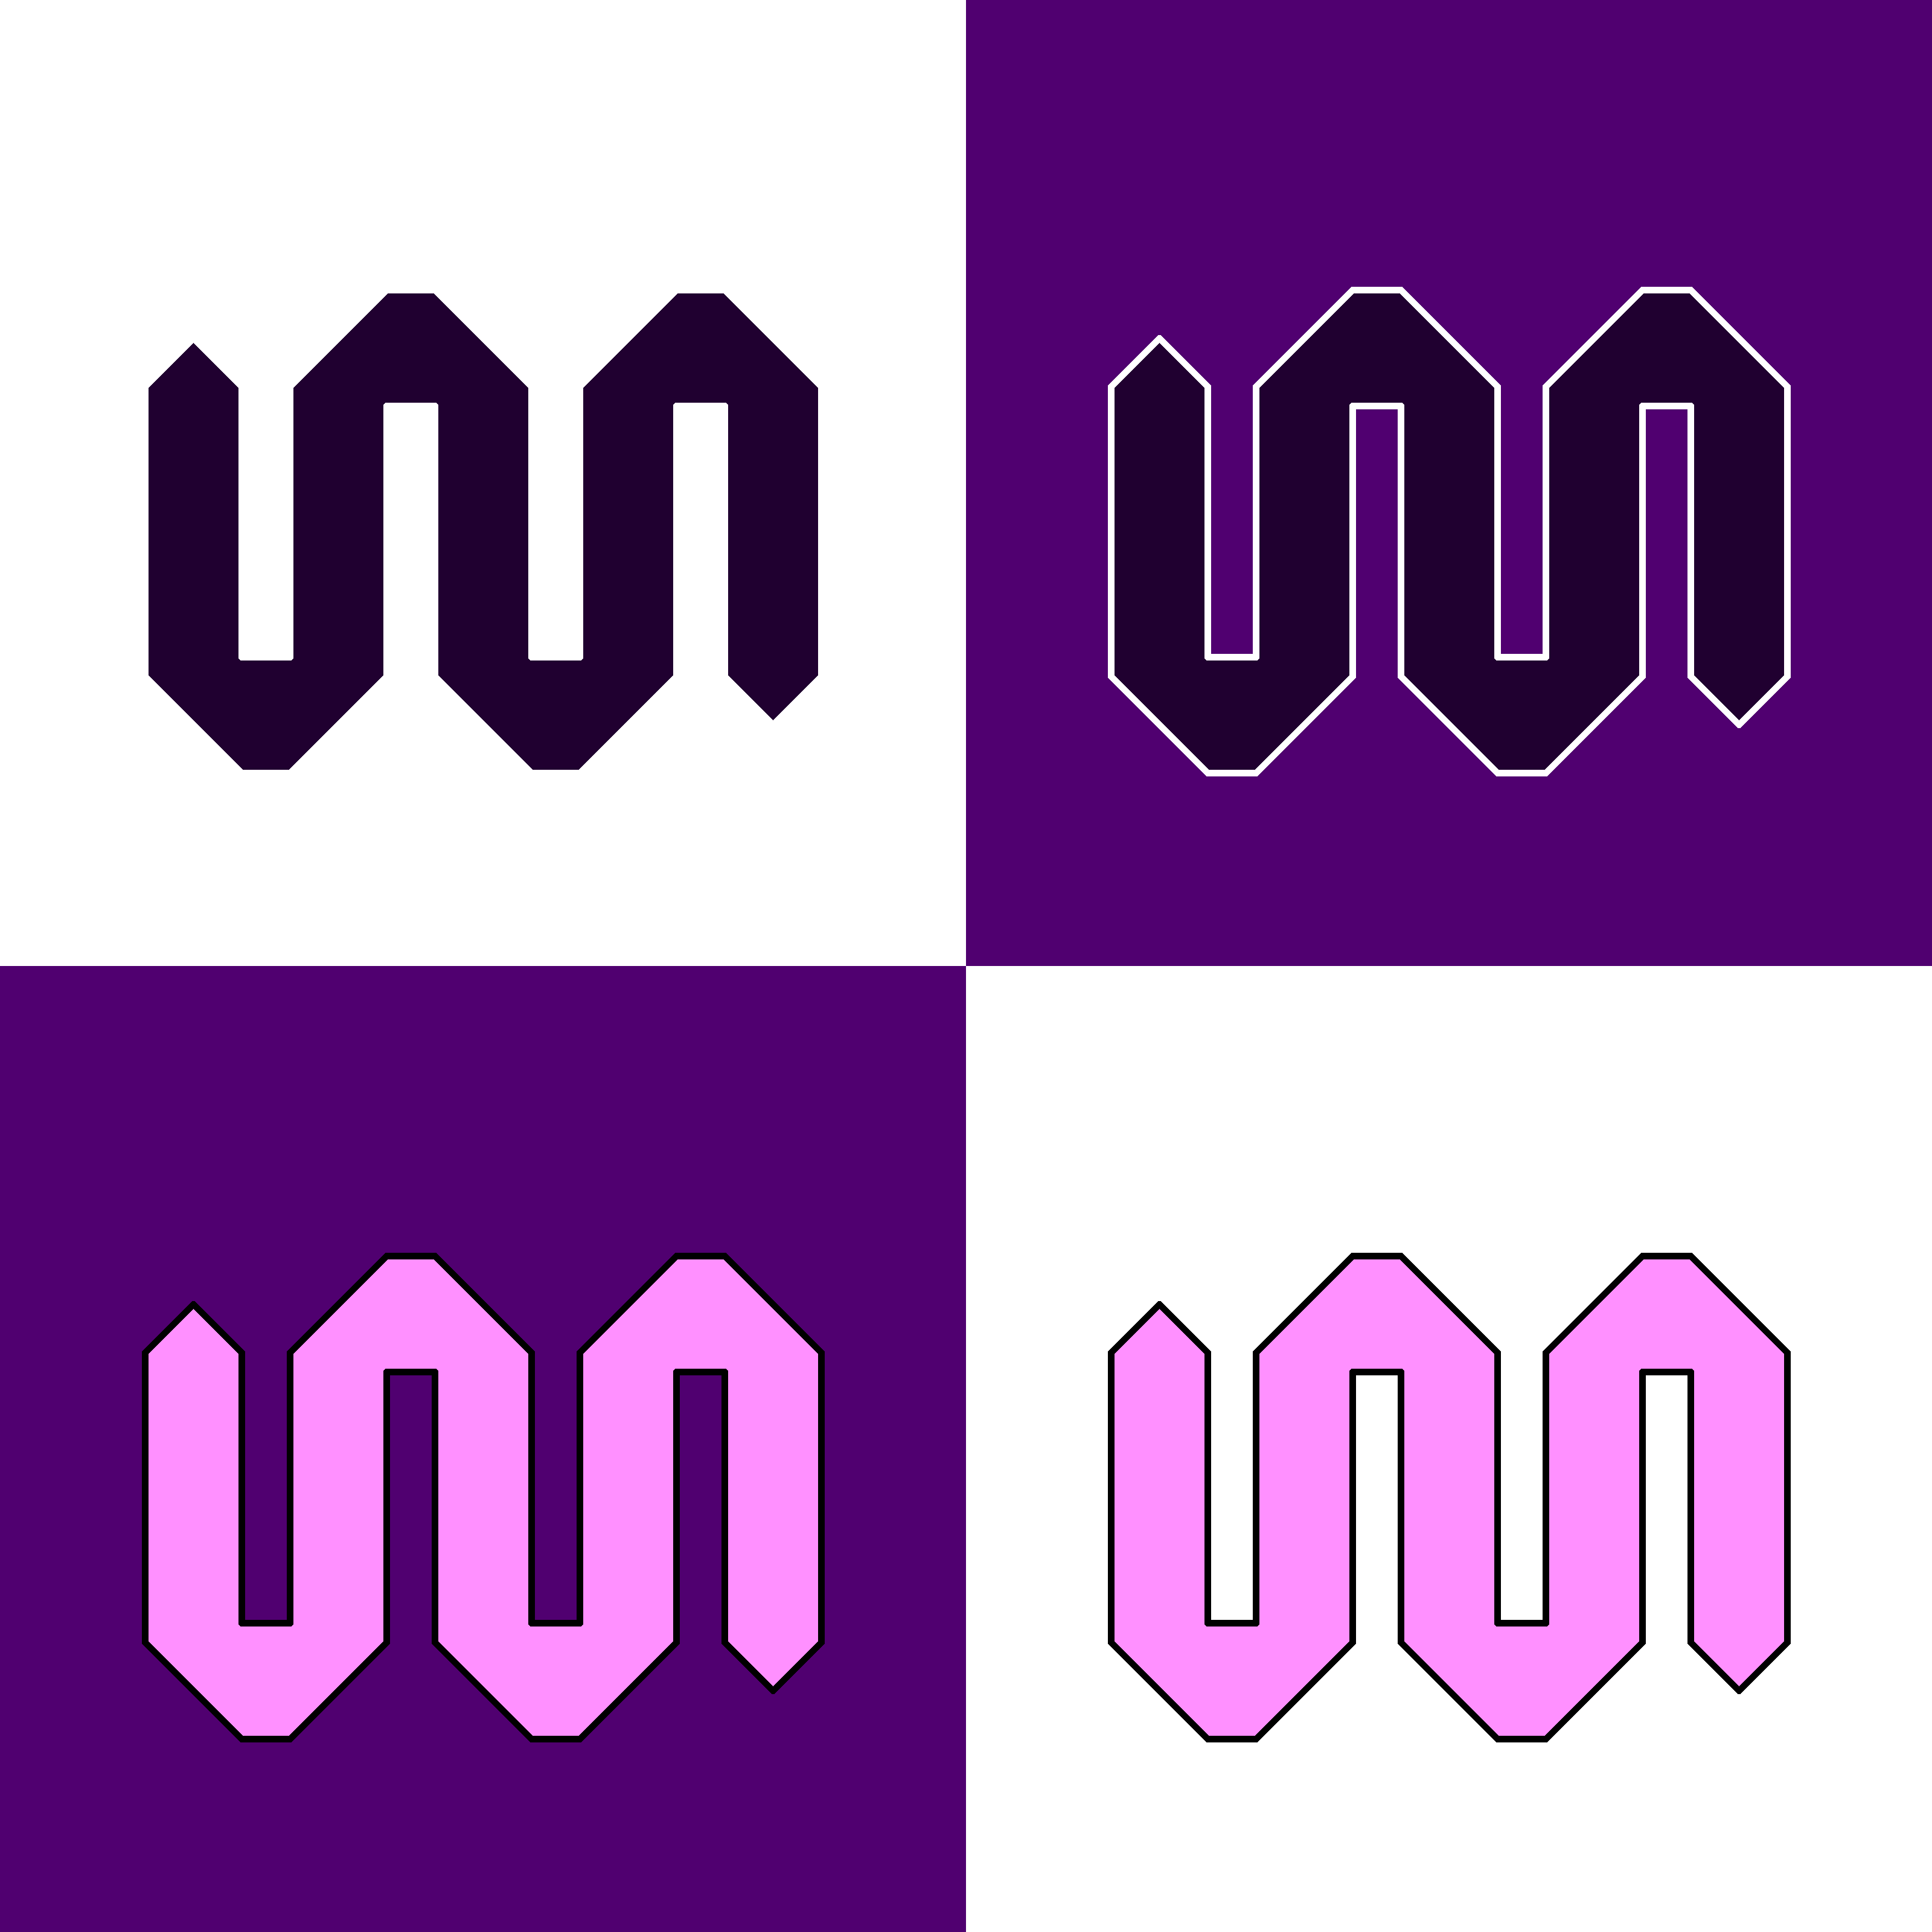
\includegraphics[width=0.4\textwidth, keepaspectratio=true]{pieces/10_wave.png}
\caption{Wave}
\label{fig:wave}
% % \centering
\end{wrapfigure}
Wave is passive piece, it has to be activated before it can move.
Activation is done in the same way as with Pyramid. Own piece
has to capture field at which Wave is located before Wave can
move.

After activation Wave moves like piece that just activated it.
Additionally, Wave can move over multiple step-fields, in the same
fashion, even if activating piece can move for only one.

\textbf{\huge{TODO :: link to "activated by/moves as" table}} % TODO :: FIX ME !!!

Pawn can activate Wave not just at its' capture-fields but also on its'
step-fields. Wave is not blocked by any piece, it can continue its'
movement freely as if there are no pieces on board at all.

Wave cannot capture any piece. Consequenly, Wave cannot check opponent's
King, and hence can't participate in a checkmate.

Wave can activate any own piece, except King. Wave can also activate
opponent's Wave.

In algebraic notation symbol for Wave is 'W'.

\clearpage % ..........................................................

\subsection*{Activation}
\addcontentsline{toc}{subsection}{Activation}

\noindent
% \begin{figure}[t]
\begin{figure}[h]
\includegraphics[width=1.0\textwidth, keepaspectratio=true]{examples/10_move_wave_init.png}
\caption{Wave activation}
\label{fig:wave_activation}
% \centering
\end{figure}

Above, Knight is about to activate Wave. After activation, Wave could
continue movement the same way Knight moves over multiple step-fields,
thus moving as if activated by Pegasus. Wave does not spend received
momentum while moving, and would transfer it entirely to piece
activated by Wave.

\clearpage % ..........................................................

\noindent
% \begin{figure}[t]
\begin{figure}[h]
\includegraphics[width=1.0\textwidth, keepaspectratio=true]{examples/10_move_wave_activated.png}
\caption{Wave activated}
\label{fig:wave_activated}
% \centering
\end{figure}

Once activated, Wave can move unhindered by surrounding pieces (green arrows),
even if they occupy step-fields in-between. Wave can also activate (red arrows)
pieces obscured by others, for instance light Pyramid which would otherwise
be out of reach for regular piece, e.g. Pegasus. Note, Wave cannot activate
Kings and opponent's pieces (grey arrows), except dark Wave.

\clearpage % ..........................................................

\subsection*{Cascading}
\addcontentsline{toc}{subsection}{Cascading}

\clearpage % ..........................................................

\subsection*{Activation by Pawn}
\addcontentsline{toc}{subsection}{Activation by Pawn}

\noindent
\begin{figure}[!h]
% \begin{figure}[!t]
\includegraphics[width=1.0\textwidth, keepaspectratio=true]{examples/10_move_wave_activation_by_pawn.png}
\caption{Wave activation by Pawns}
\label{fig:wave_activation_by_pawns}
% \centering
\end{figure}

Pawns can activate Waves on own capture-field giving it 1 momentum (1).
Pawns can also activate Waves on step-fields, giving it count of traveled-over
step-fields as momentum. For Pawn 2 that would be 1 momentum, while for Pawn 3
that would be 3.

\clearpage % ..........................................................

\section*{Initial setup}
\addcontentsline{toc}{section}{Initial setup}

Initial setup can be seen in image below:

\noindent
% \begin{figure}[t]
\begin{figure}[h]
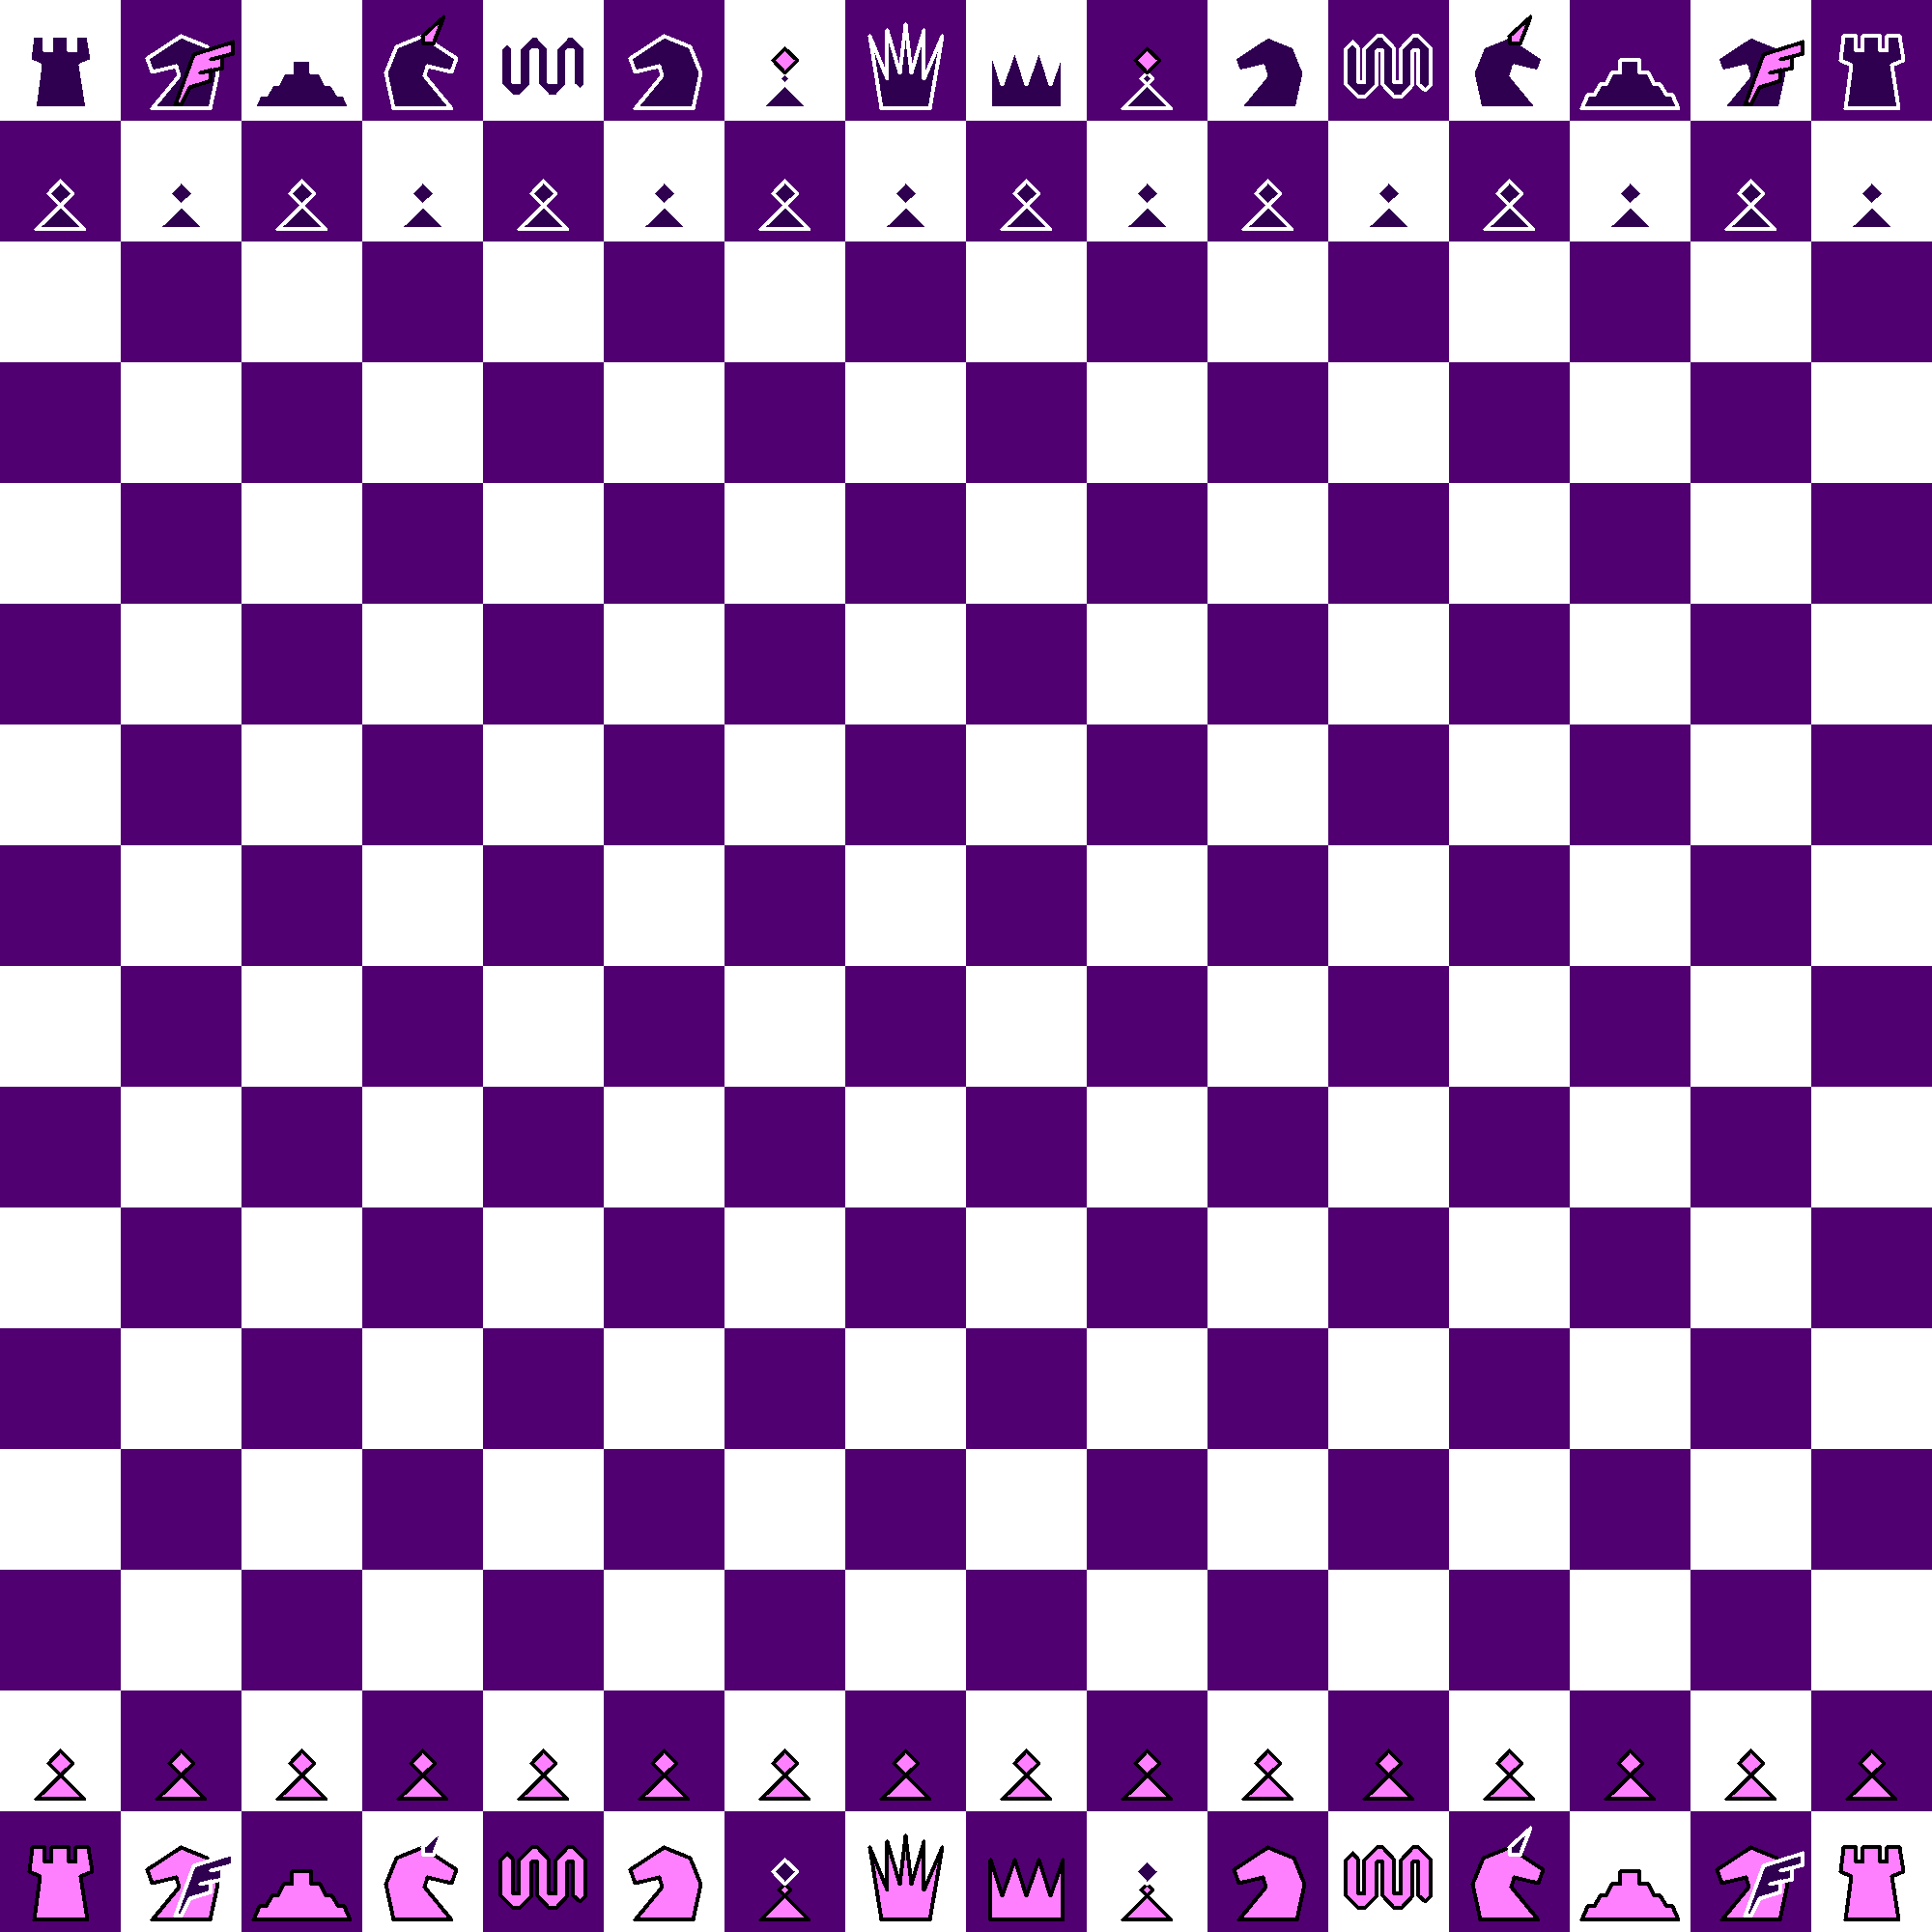
\includegraphics[width=1.0\textwidth, keepaspectratio=true]{boards/10_miranda_s_veil.png}
\caption{Miranda's veil board}
\label{fig:miranda_s_veil}
% \centering
\end{figure}

\clearpage % ..........................................................
% ---------------------------------------------- Miranda's veil chapter
